\section{Durchführung}
Zunächst wird in Abbildung \ref{fig:Messaparatur1} der Aufbau der Versuchsapparatur gezeigt.
\begin{figure}[h]
\begin{center}
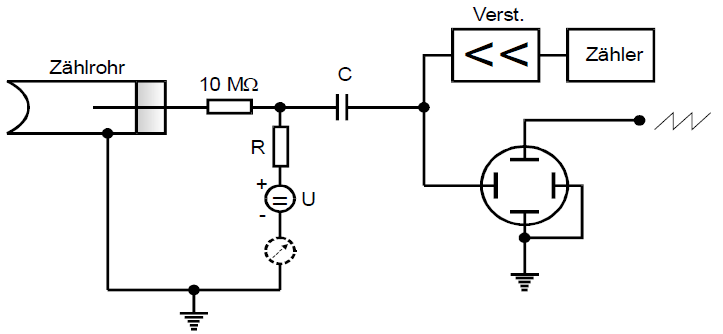
\includegraphics[width = 9cm, height= 7cm]{Messapparatur.png}
\caption{Schaltskizze des Versuchaufbaus.[1]}
\label{fig:Messaparatur1}
\end{center}
\end{figure}
\newpage
\noindent
Auf dem Zähldraht wird die Ladung $Q$ gesammelt und fließt über den Widerstand $R$ ab.
Dabei wird ein Spannungsimpuls erzeugt, der am Kondensator $C$ aufgenommen wird und im Impulszähler registriert wird.
Mithilfe eines Oszillographen werden diese Impulse sichtbar dargestellt.

\subsection{Messung der Charakteristik des Zählrohres}
Für die Messung wird eine $\beta$-Quelle vor dem Endfensterzählrohr platziert.
Mit diesem Aufbau wird der Zusammenhang der Zählrate von der Spannung ($\SI{300}{V}$-$\SI{700}{V}$) und dem mittleren Zählrohrstrom $\overline{I}$ ermittelt.
Die freigesetzte Ladungsmenge wird durch den mittleren Zählrohrstrom bestimmt. Es gilt
\begin{align}
\Delta {Q} = \frac{\overline{{I}}\Delta {t}}{{Z}} \,.
\end{align}
Dabei ist $\Delta t$ die Messzeit und $Z$ die Zählrate.
  Es werden 40 Messungen in einem Intervall von $\SI{60}{s}$ durchgeführt.
\subsection{Die Nachentladungen}
Der Abstand zwischen $\beta$-Quelle und Zählrohr bleibt unverändert und der Ladungsimpuls für $\SI{350}{V}$ und $\SI{700}{V}$ werden auf dem Oszilloskop betrachtet.
Die Kurve aus Abbildung 3 entsteht auf dem Display.
\label{ssec:Nachentladung}
\subsection{Die Totzeit und Erholungszeit}
Die Totzeit wird über 2 Methoden ermittelt,
die oszillosgraphische Darstellung und die Zwei-Quell-Methode.
Für die erste Methode werden drei Messungen mit $\SI{450}{V}$, $\SI{550}{V}$ und $\SI{650}{V}$ aufgenommen.
Es wird, wie in Abschnitt \ref{ssec:Nachentladung} "Die Nachentladung" beschrieben, vorgegangen.
Die Totzeit und die Erholungszeit werden ermittelt. \\
Für die zweite Methode werden ebenfalls des drei Messungen vorgenommen. Bei gleichbleibender Betriebsspannung von $\SI{450}{V}$
wird zunächst die Impulsrate von $N_{\text{1}}$ untersucht.
Dann wird eine zweite, schwächere $\beta$-Quelle hinzugefügt und die Impulsraten beider Quellen werden gemessen.
Im letzten Schritt wird lediglich die Impulsrate $N_{\text{2}}$ der zweiten Quelle gemessen.
Um die Richtigkeit zu überprüfen, muss folgende Bedingung
\begin{align}
   {N}_{1+2} < {N}_1 + {N}_2
\end{align}
gelten. Aus den ermittelten Daten errechnet sich die gesuchte Totzeit näherungsweise durch
\begin{align} 
    {T} \approx \frac{{N}_1+{N}_2-{N}_{1+2}}{2{N}_1{N}_2} \,.
\end{align}
\label{sec:Durchführung}

